\documentclass{article}
\usepackage{graphicx}
\usepackage{subcaption}
\usepackage{float}
\usepackage{amsmath}
\usepackage{natbib}
\usepackage[french]{babel}
\usepackage[T1]{fontenc}
\usepackage[utf8]{inputenc}
\usepackage{hyperref}

\usepackage[french]{babel}
\usepackage[utf8]{inputenc}
\usepackage{hyperref} % Pour les liens internes
\usepackage{graphicx}
\usepackage[numbers]{natbib}
\usepackage{amsmath}
\usepackage{float} % Pour mieux gérer les positions des images
\usepackage{geometry} % Pour les marges
\usepackage{parskip} % Pour espacer les paragraphes
\usepackage{xcolor} % Pour ajouter de la couleur
\usepackage{amssymb}

\geometry{top=1in, bottom=1in, left=1in, right=1in} % Marges personnalisées
\setlength{\parskip}{1em} % Espacement entre les paragraphes
\setlength{\parindent}{0pt} % Pour éviter l'indentation des paragraphes

%%%%%%%%%%%%%%%% Lengths %%%%%%%%%%%%%%%%
\setlength{\textwidth}{15.5cm}
\setlength{\evensidemargin}{0.5cm}
\setlength{\oddsidemargin}{0.5cm}

%%%%%%%%%%%%%%%% Variables %%%%%%%%%%%%%%%%
\def\projet{5}
\def\titre{Interpolation polynomial}
\def\groupe{3}
\def\equipe{3}
\def\responsible{Soufiane SBAI}
\def\secretary{Florian Arnoud}
\def\others{Toine Horny Joan Dumarchat}

\begin{document}

%%%%%%%%%%%%%%%% Header %%%%%%%%%%%%%%%%
\noindent\begin{minipage}{0.98\textwidth}
  \vskip 0mm
  \noindent
  { \begin{tabular}{p{7.5cm}}
      {\bfseries \sffamily
        Projet \projet} \\ 
      {\itshape \titre}
    \end{tabular}}
  \hfill 
  \fbox{\begin{tabular}{l}
      {~\hfill \bfseries \sffamily Groupe \groupe\ - Equipe \equipe
        \hfill~} \\[2mm] 
      Responsable : \responsible \\
      Secrétaire : \secretary \\
      Codeurs : \others
    \end{tabular}}
  \vskip 4mm ~

  ~~~\parbox{0.95\textwidth}{\small \textit{Résumé~:} \sffamily  L’objectif de ce projet est de modéliser l’écoulement de l’air autour d’un profil d’aile et d’en déduire 
  une carte de pression au-dessus et en dessous de l’aile. Cette analyse permettra d’estimer la portance générée par le profil étudié.Pour ce faire, deux étapes
   préliminaires sont nécessaires l'interpolation du profil de l'aile par la méthode des spline cubiques, puis la méthode d'intégration.}
  \vskip 1mm ~
\end{minipage}


\section{Interpolation par la méthode du spline cubique}
\subsection{Calcul des coefficients $y''_i$}
La première étape de l'interpolation par spline cubique consiste à calculer les coefficients $y''_i$. Pour cela, il est nécessaire de résoudre le système d'équations suivant : \( A V = B \), où :

\[
\small
A =
\begin{bmatrix}
\frac{h_0 + h_1}{3} & \frac{h_1}{6} & & & & \\
\frac{h_1}{6} & \frac{h_1 + h_2}{3} & \frac{h_2}{6} & & & \\
& \ddots & \ddots & \ddots & & \\
& & \frac{h_{i-1}}{6} & \frac{h_{i-1} + h_i}{3} & \frac{h_i}{6} & \\
& & & \ddots & \ddots & \ddots \\
& & & & \frac{h_n}{6} & \frac{h_n}{3}
\end{bmatrix}
\normalsize
\]

(A matrice tridiagonale symétrique)

\[
V = \begin{bmatrix}
y_1'' & y_2'' & \cdots & y_{n-1}''
\end{bmatrix}
\quad \text{et} \quad
B = \begin{bmatrix}
\frac{y_2 - y_1}{h_1} - \frac{y_1 - y_0}{h_0} &
\frac{y_3 - y_2}{h_2} - \frac{y_2 - y_1}{h_1} &
\cdots &
\frac{y_n - y_{n-1}}{h_n} - \frac{y_{n-1} - y_{n-2}}{h_{n-1}}
\end{bmatrix}
\]

\subsection{Approximation de $f$ par $\omega_i(x)$}
La seconde partie consiste à approximer $f(x)$ par $\omega_i(x)$. Tout d'abord, nous devons déterminer l'intervalle dans lequel se trouve $x$ ($x \in [x_i, x_{i+1}]$), puis évaluer $\omega_i(x)$ à partir de la formule suivante :

\[
\omega_{|x_i;x_{i+1}}(x) = A_i(x) y_i + B_i(x) y_{i+1}
+ \frac{h_i^2}{6} \left( y_i'' \left( A_i^1(x) - A_i(x) \right) + y_{i+1}'' \left( B_i^1(x) - B_i(x) \right) \right)
\]

\subsection{Précision de l'implémentation}
L'implémentation permet une approximation précise pour des fonctions telles que la \textbf{fonction cube} (Figure 1(a)) et le \textbf{sinus} (Figure 1(b)). De plus, l'implémentation donne de bons résultats pour l'approximation de la fonction représentant \textbf{l'aile d'un avion} (Figure 1(c)).

\begin{figure}[H]
  \centering
  \begin{subfigure}[b]{0.3\textwidth}
    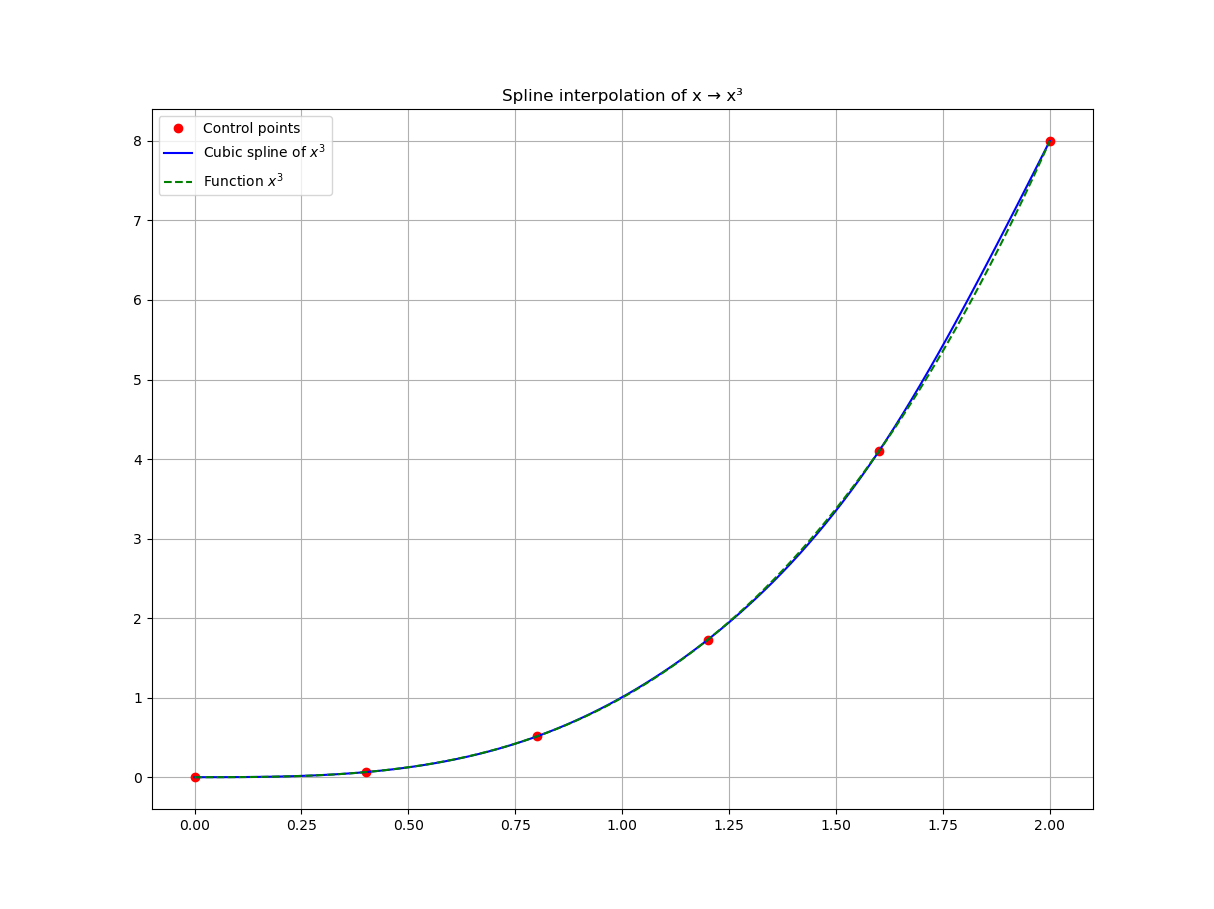
\includegraphics[width=\textwidth]{img/Cubic_visualisation.png}
    \caption{Fonction cube}
    \label{fig:cube}
  \end{subfigure}
  \hfill
  \begin{subfigure}[b]{0.3\textwidth}
    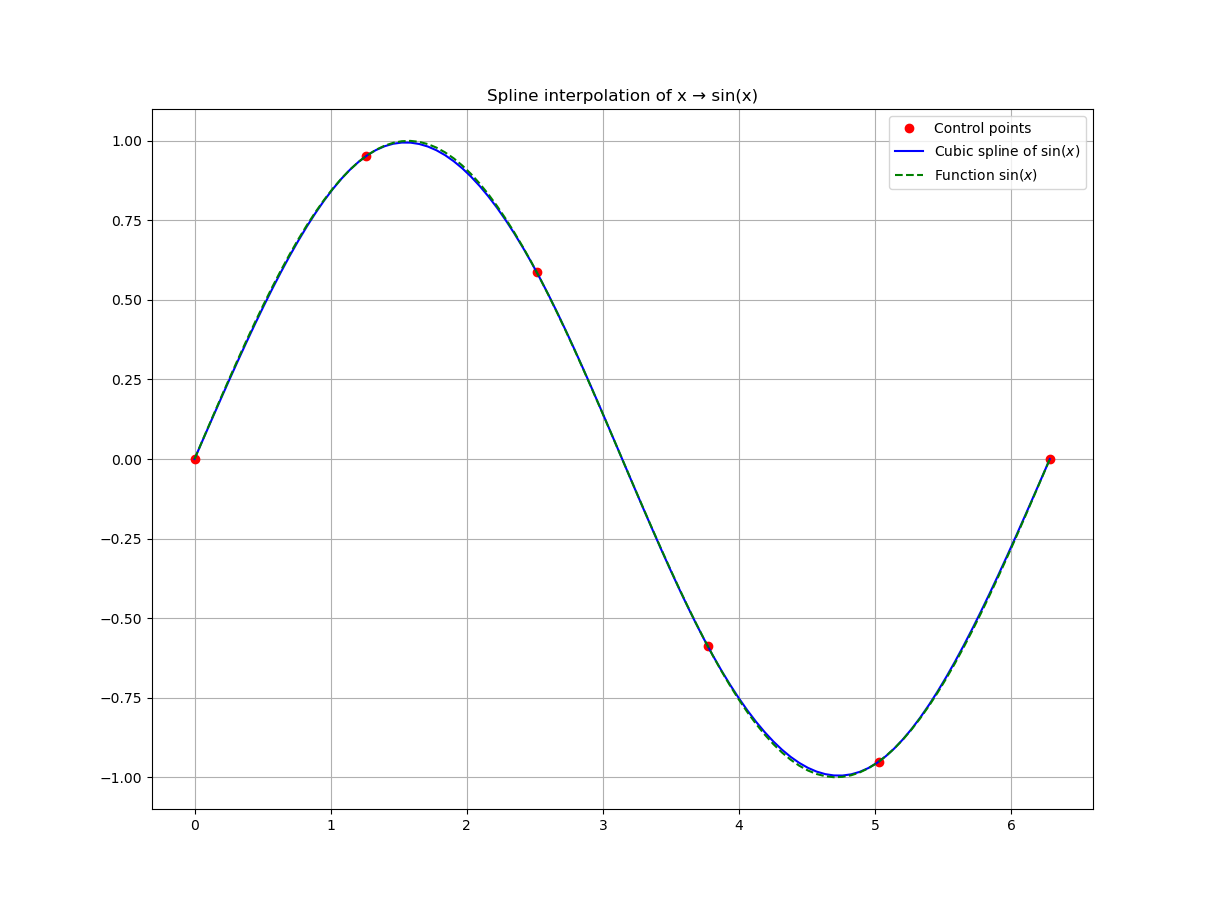
\includegraphics[width=\textwidth]{img/Sin_visualisation.png}
    \caption{Sinus}
    \label{fig:sinus}
  \end{subfigure}
  \hfill
  \begin{subfigure}[b]{0.3\textwidth}
    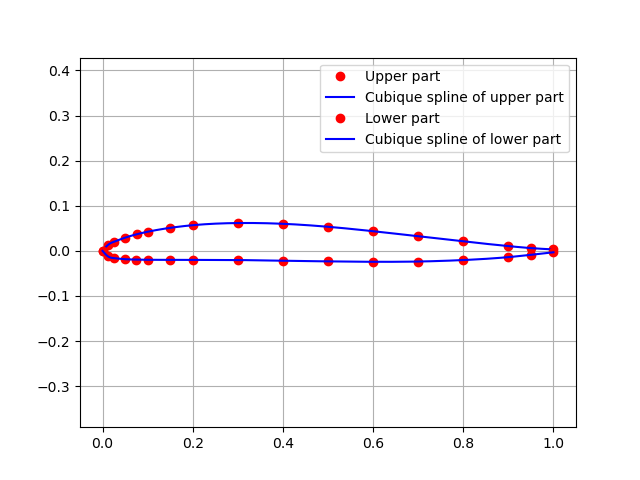
\includegraphics[width=\textwidth]{img/Airfoil_visualisation.png}
    \caption{Aile d’un avion}
    \label{fig:airflow}
  \end{subfigure}
  \caption{Illustrations des trois concepts}
\end{figure}

\section{Implémentation de l'intégration pour le calcul de longueur}
La deuxième partie préliminaire de l'implémentation consiste à développer une méthode d'intégration permettant de calculer la longueur d'un flux d'air selon l'équation suivante :

\[
L([0;T]) = \int_{0}^{T} \sqrt{1 + (f'(x))^2} \,dx
\]

Plusieurs méthodes d'intégration ont été implémentées.

\subsection{Méthode des rectangles et des trapèzes}
La première méthode "naïve" consiste à approximer l'intégrale par la méthode des rectangles, qui divise l'aire sous la courbe en une succession de découpes rectangulaires (à gauche ou à droite) :

\[
\int_{\alpha_{i-1}}^{\alpha_i} f(t) \, dt \approx (\alpha_i - \alpha_{i-1}) \times f(\alpha_{i-1})
\]

ou à droite :

\[
\int_{\alpha_{i-1}}^{\alpha_i} f(t) \, dt \approx (\alpha_i - \alpha_{i-1}) \times f(\alpha_i)
\]

Cela nous donne l'approximation :

\[
I_{R} = \int_{a}^{b} f(t) \, dt \approx h \sum_{i=1}^{n} f(a + i h)
\]

Ces deux méthodes sont des approximations d'ordre 0. Il est possible d'améliorer l'approximation en utilisant la méthode des rectangles avec le point milieu, ce qui donne :

\[
I_{R_m} = \int_{a}^{b} f(t) \, dt \approx h \sum_{i=0}^{n-1} f \left( a + ih + \frac{h}{2} \right)
\]

Une autre méthode consiste à utiliser les trapèzes, qui donne une approximation d'ordre 1 :

\[
I_T = \int_a^b f(t) \, dt \approx h \left( \frac{f(a) + f(b)}{2} + \sum_{i=1}^{n-1} f(a + ih) \right)
\]

\subsection{Méthode d'intégration itérative}
Pour améliorer la précision des méthodes d'intégration numérique, on utilise des schémas de raffinement en doublant le nombre de subdivisions, tout en réutilisant les calculs précédents pour insérer de nouveaux points intermédiaires.

Les formules suivantes donnent une mise à jour efficace de l'approximation lorsque le pas \( h \) est divisé par 2 (ou 3 dans le cas du point milieu) :

\begin{itemize}
  \item \textbf{Rectangles et trapèzes} :
  \[
  I(2n) = \frac{1}{2} I(n) + \frac{h}{2} \sum_{k=0}^{n-1} f\left( a + hk + \frac{h}{2} \right)
  \]
  \item \textbf{Point milieu (triplement du pas)} :
  \[
  I_{Rm}(3n) = \frac{1}{3} I_{Rm}(n) + \frac{h}{3} \sum_{k=0}^{n-1} \left[ f\left( a + hk + \frac{h}{6} \right) + f\left( a + hk + \frac{5h}{6} \right) \right]
  \]
  \item \textbf{Simpson} :
  \[
  I_S(n) = h \left( I_0 + \frac{1}{3} I_1(n) + \frac{2}{3} I_2(n) \right)
  \]
  avec les récurrences :
  \[
  I_1(2n) = I_1(n) + I_2(n), \quad
  I_2(2n) = 2 \sum_{i=0}^{n-1} f\left( a + i \frac{h}{2} + \frac{h}{4} \right)
  \]
\end{itemize}

\subsection{Analyse des précisions et vitesses de convergence}
La précision des méthodes d'intégration numérique dépend de la régularité de la fonction \( f \) et du pas \( h \). Voici une analyse des erreurs associées aux différentes méthodes :

\begin{itemize}
  \item \textbf{Rectangles et trapèzes} : erreur en \( \mathcal{O}(h) \) pour les rectangles droit et gauche, et \( \mathcal{O}(h^2) \) pour le point milieu et les trapèzes.
  \item \textbf{Point milieu} : erreur en \( \mathcal{O}(h^2) \), souvent plus précise que les rectangles.
  \item \textbf{Simpson} : erreur en \( \mathcal{O}(h^4) \), donc beaucoup plus précise que les autres méthodes.
\end{itemize}

Ainsi, la méthode de Simpson offre un gain significatif en précision pour un même nombre de points, à condition que \( f \) soit suffisamment dérivable.

\begin{figure}[h!]
  \centering
  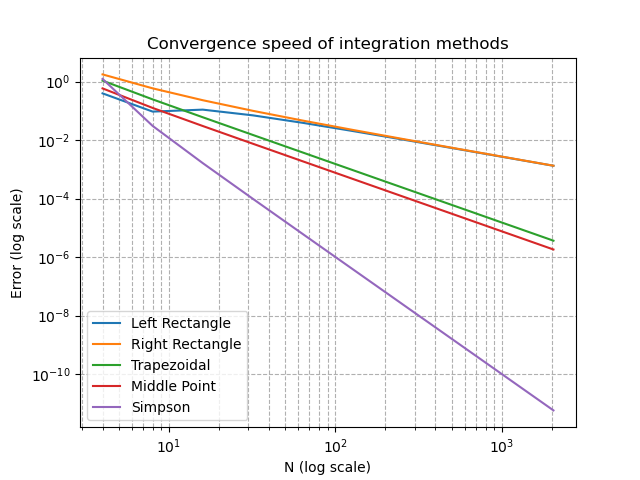
\includegraphics[width=0.5\textwidth]{img/Intregral_convergence.png}
  \caption{Comparaison des vitesses de convergence des différentes méthodes d'intégration.}
  \label{fig:convergence}
\end{figure}

\newpage 

\section{Application sur la modélisation du flux d'air sur le profil d'une aile}

Dans cette section, nous appliquons la méthode d'interpolation par spline cubique pour modéliser le flux d'air sur le profil d'une aile. Le profil de l'aile est représenté par un ensemble de points mesurés le long de la surface de l'aile, et l'objectif est de trouver une courbe lisse qui représente ce profil.

\subsection{Description du problème}
Le flux d'air est modélisé en utilisant les données expérimentales obtenues à partir de mesures sur le profil d'une aile d'avion. Les points de données représentent les coordonnées de la surface de l'aile en fonction de la position le long de l'axe de l'aile. Ces données sont utilisées pour interpoler une fonction continue qui représente la forme du profil.

Les données sont présentées sous la forme d'une série de points $(x_i, y_i)$ où $x_i$ est la position le long de l'axe de l'aile et $y_i$ est la hauteur correspondante du profil.


\subsection{Résultats de l'application}
En appliquant l'interpolation par spline cubique aux données expérimentales du profil de l'aile, nous obtenons une courbe lisse qui représente le profil de l'aile, ainsi que les flux d'air autour du profil de l'aile. (Figures 3 et 4)

\begin{figure}[H]
  \centering
  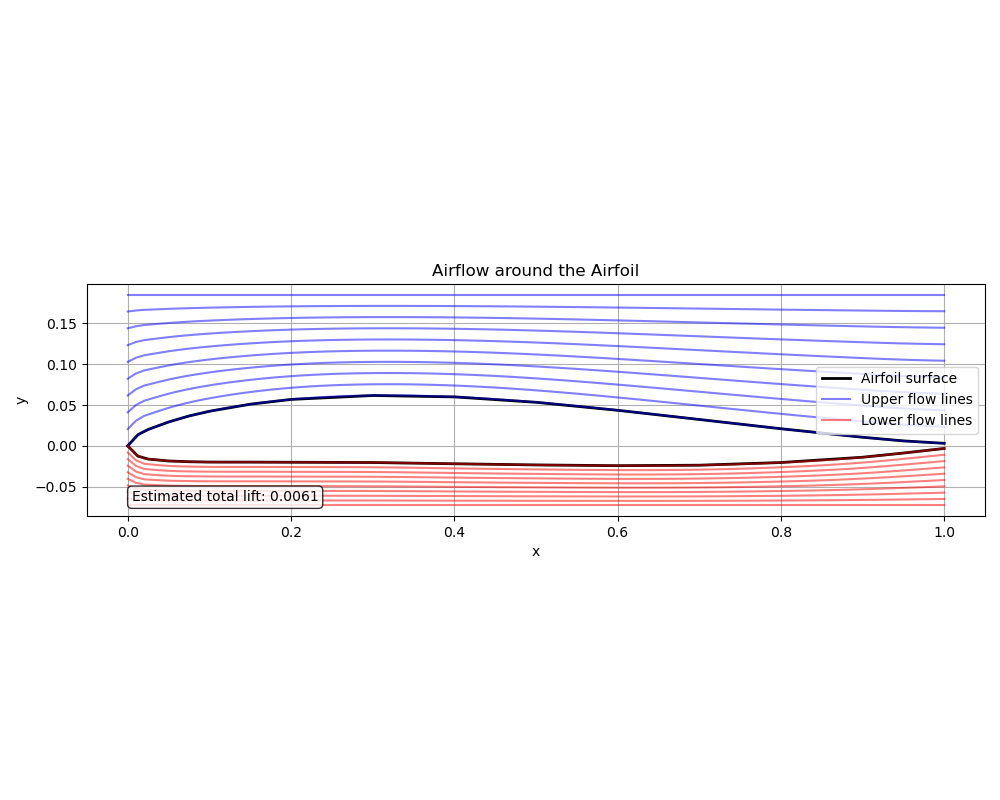
\includegraphics[width=0.5\textwidth]{img/airflow_visualisation.png}
  \caption{Profil de l'aile après interpolation par spline cubique}
  \label{fig:foil_profil}
\end{figure}

\begin{figure}[H]
  \centering
  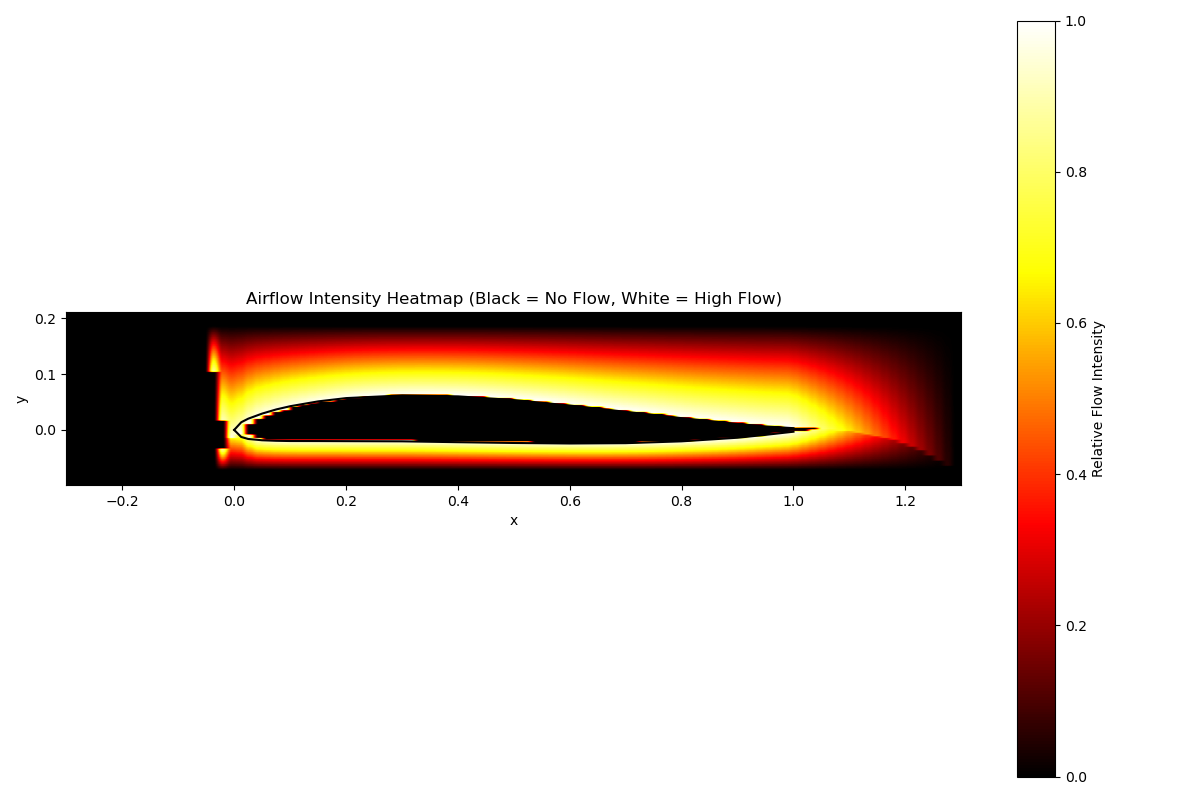
\includegraphics[width=0.5\textwidth]{img/pressure_map.png}
  \caption{Pressure map avec gradient du profil de l'aile}
  \label{fig:pressure_map}
\end{figure}

\subsection{Conclusion}
L'interpolation par spline cubique permet d'obtenir une approximation lisse du profil de l'aile à partir des données expérimentales. Cette méthode permet de maintenir la continuité des dérivées premières et secondes. Ce qui dans notre cas permet d'avoir une visualisation des pressions autour du profil de l'aile.

\end{document}
    